Aus den in der Business Process Discovery Phase gesammelten unstrukturierten Daten müssen in einem nächsten Schritt strukturierte Prozessmodelle erstellt werden, die als Grundlage für die weitere Analyse dienen.
Zur Modellierung von Geschäftsprozessen gibt es verschiedene Ansätze, die im Folgenden vorgestellt werden.

\subsubsection{UML}
Die Unified Modeling Language (UML) ist ein Standardset vob Regeln für grafische Modellierung, die für die Softwareentwicklung und das Systemdesign entwickelt wurden und die Darstellung und Dokumentation der Struktur und des Verhaltens von Systemen ermöglicht~\cite{OMG2017}.
Im Zusammenhang mit der Prozessmodellierung können insbesondere Aktivitätsdiagramme verwendet werden, um Prozesse in Aktionen aufgeteilt darzustellen. Dabei werden verschiedene Akteure durch sogenannte Swimlanes repräsentiert~\cite{List2006}.\\

Allerdings hat die UML bei der Modellierung von Geschäftsprozessen gewisse Einschränkungen.
Während sie umfassende Unterstützung für Kontrollfluss- und Datenperspektiven bietet, ist ihre Anwendbarkeit auf ressourcenbezogene oder organisatorische Aspekte begrenzt~\cite{Russell2006}.
Darüber hinaus kann man mit UML Schwierigkeiten haben, einige natürliche Konstrukte zu erfassen, die in Geschäftsprozessen vorkommen, wie z. B. Fälle und Interaktionen mit der betrieblichen Umgebung~\cite{Russell2006}.


\subsubsection{BPMN (Business Process Model and Notation)}

Die Business Process Model and Notation (BPMN) 2.0 ist eine standardisierte Modellierungssprache, die verwendet wird, um Geschäftsprozesse grafisch darzustellen.
BPMN 2.0 wurde von der Object Management Group (OMG) entwickelt und bietet eine einheitliche Sprache, um Prozesse und Aktivitäten in Unternehmen zu beschreiben.\\
Das BPMN 2.0-Schema besteht aus einer Vielzahl von Symbolen, die zur Darstellung von Ereignissen, Aktivitäten, Gateways, Datenobjekten und weiteren Konstrukten verwendet werden.
Diese Symbole werden in einer grafischen Notation angeordnet, um einen Prozessfluss zu erzeugen, der die verschiedenen Schritte des Prozesses und deren Beziehungen zueinander widerspiegelt.

\begin{enumerate}[label=\arabic*., leftmargin=*]
    \item \textbf{Flow Objects}: Dies sind die wichtigsten grafischen Elemente, die zur Definition des Prozessverhaltens verwendet werden. Flow Objects werden in drei Typen unterteilt:
    \begin{enumerate}
        \item[] \begin{minipage}{\linewidth}
            \textbf{Events}: Kreise, die Ereignisse darstellen, die einen Prozess auslösen oder daraus resultieren können. Sie können Start-, Zwischen- oder Endereignisse sein.
            \begin{center}
                \begin{tikzpicture}[baseline=-0.5ex]
                    % Events
                    \node[draw, circle, minimum size=1cm] (start) {Start};
                    \node[draw, circle, double, minimum size=1cm, right=1cm of start] (intermediate) {Int.};
                    \node[draw, circle, minimum size=1cm, right=1cm of intermediate, line width=2pt] (end) {End};
                \end{tikzpicture}
            \end{center}
        \end{minipage}
    
        \item[] \begin{minipage}{\linewidth}
            \textbf{Activities}: Abgerundete Rechtecke, die die im Prozess ausgeführte Arbeit darstellen. Aktivitäten können Aufgaben oder Unterprozesse sein.
            \begin{center}
                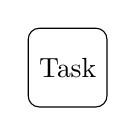
\begin{tikzpicture}[baseline=-0.5ex]
                    % Task
                    \node[draw, rectangle, rounded corners, minimum size=1cm] (task) {Task};
                    \end{tikzpicture}
            \end{center}
        \end{minipage}
        
        \item[] \begin{minipage}{\linewidth}
            \textbf{Gateways}: Rauten, die Entscheidungspunkte oder Gabelungen und Zusammenführungen von Pfaden im Prozess darstellen. Sie werden verwendet, um den Prozessfluss zu steuern.
            \begin{center}
                \begin{tikzpicture}[baseline=-0.5ex]
                    % Gateway
                    \node[draw, diamond, aspect=2, minimum size=1cm] (gateway) {};
                    \end{tikzpicture}
            \end{center}
        \end{minipage}
    \end{enumerate}

    \item \textbf{Verbindungsobjekte}: Dies sind die Elemente, die Flow-Objekte verbinden und die Reihenfolge des Prozesses oder des Nachrichtenflusses zwischen den Teilnehmern anzeigen. Zu den verbindenden Objekten gehören:
    \begin{enumerate}
        \item[] \begin{minipage}{\linewidth}
            \textbf{Sequence Flow:} Durchgehende Pfeile, die die Reihenfolge anzeigen, in der Aktivitäten, Ereignisse und Gateways ausgeführt oder ausgewertet werden.
            \begin{center}
            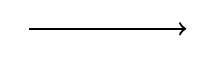
\begin{tikzpicture}[baseline=-0.5ex]
                % Sequence Flow
                \draw[->, thick] (0, 0) -- (2, 0);
            \end{tikzpicture}
            \end{center}
        \end{minipage}

        \item[] \begin{minipage}{\linewidth}
            \textbf{Message Flow:} Gestrichelte Pfeile, die den Austausch von Nachrichten zwischen den Teilnehmern eines Prozesses anzeigen.
            \begin{center}
                \begin{tikzpicture}[baseline=-0.5ex]
                    % Message Flow
                    \draw[dashed, ->] (0, 0) -- (2, 0);
                    \draw (0, 0) circle [radius=1.5pt];
                \end{tikzpicture}
                \end{center}
            \end{minipage}
        
        \item[] \begin{minipage}{\linewidth}
            \textbf{Association:} Gestrichelte Linien, die Daten, Anmerkungen oder Artefakte mit Flow-Objekten verbinden.
            \begin{center}
                \begin{tikzpicture}[baseline=-0.5ex]
                    % Association
                    \draw[dotted] (0, 0) -- (2, 0);
                \end{tikzpicture}
            \end{center}
        \end{minipage}
    \end{enumerate}

    \item \textbf{Swimlanes}: Diese Elemente werden verwendet, um den Prozess visuell zu organisieren und in verschiedene Rollen, Verantwortlichkeiten oder Funktionsbereiche zu unterteilen. Swimlanes umfassen:
    \begin{enumerate}
        \item[] \begin{minipage}{\linewidth}
            \textbf{Pools:} Rechtecke, die die an einem Prozess beteiligten Personen darstellen. Ein Pool kann eine oder mehrere Bahnen enthalten.
            \begin{center}
            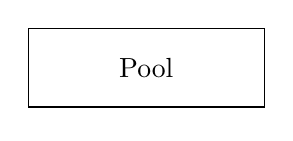
\begin{tikzpicture}[baseline=-0.5ex]
                % Pool
                \draw (0, 0) rectangle (3, 1);
                \node at (1.5, 0.5) {Pool};
            \end{tikzpicture}
            \end{center}
        \end{minipage}
        
        \item[] \begin{minipage}{\linewidth}
            \textbf{Lanes:} Unterabteilungen innerhalb eines Pools. Lanes helfen dabei, den Prozess auf der Grundlage von Rollen oder Funktionsbereichen innerhalb eines Teilnehmers weiter zu organisieren und zu kategorisieren.
            \begin{center}
            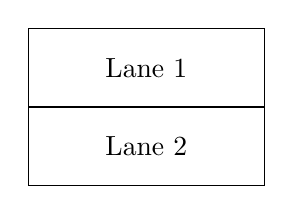
\begin{tikzpicture}[baseline=-0.5ex]
                % Lanes
                \draw (0, 0) rectangle (3, 2);
                \draw (0, 1) -- (3, 1);
                \node at (1.5, 1.5) {Lane 1};
                \node at (1.5, 0.5) {Lane 2};
            \end{tikzpicture}
            \end{center}
        \end{minipage}
    \end{enumerate}

    \item \textbf{Artifacts}: Diese Elemente liefern zusätzliche Informationen über den Prozess, die nicht direkt mit der Sequenz oder dem Nachrichtenfluss verbunden sind. Zu den Artefakten gehören:
    \begin{enumerate}
        \item[] \begin{minipage}{\linewidth}
            \textbf{Input Data Objects:} Icons, die Dateneingaben im Prozess darstellen.
            \begin{center}
                \begin{tikzpicture}[baseline=-0.5ex]
                    % Input Data Object
                    \draw (0, 0) -- (1, 0) -- (1, 1.3) -- (0.9, 1.4) -- (0, 1.4) -- (0, 0);
                    \node[single arrow, draw, minimum height=0.4cm, minimum width=0.4cm, anchor=west, yscale=0.4, single arrow head extend=0.1cm] at (0.1, 1.15) {};
                    \node at (0.5, 0.7) {IDO};
                \end{tikzpicture}
            \end{center}
        \end{minipage}
    
        \item[] \begin{minipage}{\linewidth}
            \textbf{Output Data Objects:} Icons, die Datenausgaben im Prozess darstellen.
            \begin{center}
                \begin{tikzpicture}[baseline=-0.5ex]
                    % Output Data Object
                    \draw (0, 0) -- (1, 0) -- (1, 1.3) -- (0.9, 1.4) -- (0, 1.4) -- (0, 0);
                    \node[single arrow, draw, minimum height=0.4cm, minimum width=0.4cm, anchor=west, yscale=0.4, single arrow head extend=0.1cm, fill=black] at (0.1, 1.15) {};
                    \node at (0.5, 0.7) {ODO};
                \end{tikzpicture}
            \end{center}
        \end{minipage}
    
        \item[] \begin{minipage}{\linewidth}
            \textbf{Data Stores:} Icons, die einen Ort darstellen, an dem Daten während der Prozessausführung gespeichert und abgerufen werden können.
            \begin{center}
            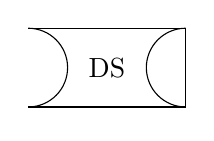
\begin{tikzpicture}[baseline=-0.5ex]
                % Data Store
                \draw (0, 0) -- (2, 0) -- (2, 1) -- (0, 1);
                \draw (0, 1) arc (90:-90:0.5);
                \draw (2, 1) arc (90:270:0.5);
                \node at (1, 0.5) {DS};
            \end{tikzpicture}
            \end{center}
        \end{minipage}
    
        \item[] \begin{minipage}{\linewidth}
            \textbf{Group:} Ein gestricheltes Rechteck, das Elemente des Prozesses visuell gruppiert und oft zu Dokumentationszwecken verwendet wird.
            \begin{center}
            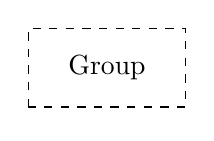
\begin{tikzpicture}[baseline=-0.5ex]
                % Group
                \draw[dashed] (0, 0) rectangle (2, 1);
                \node at (1, 0.5) {Group};
            \end{tikzpicture}
            \end{center}
        \end{minipage}
    
        \item[] \begin{minipage}{\linewidth}
            \textbf{Text Annotations:} Eine Klammer, die es ermöglicht Kommentare oder Beschreibungen zu jedem Teil des Prozesses hinzuzufügen.
            \begin{center}
            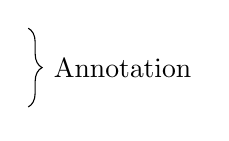
\begin{tikzpicture}[baseline=-0.5ex]
                % Text Annotation
                \draw[decorate, decoration={brace, amplitude=5pt, mirror}] (0, 0) -- (0, 1);
                \node[anchor=west] at (0.2, 0.5) {Annotation};
            \end{tikzpicture}
            \end{center}
        \end{minipage}
    \end{enumerate}
\end{enumerate}

\subsubsection{Event-driven Process Chain (EPC)}
EPC ist ein Prozessmodellierungskonzept, das auf der Idee basiert, dass Prozesse aus einer Reihe von Ereignissen und Funktionen bestehen.
EPCs bieten eine grafische Darstellung, die es erlaubt, den Prozessfluss auf eine visuelle und verständliche Art darzustellen.
Die Methode wird häufig eingesetzt, da sie es ermöglicht, die Abhängigkeiten zwischen Prozessschritten einfach abzubilden und somit die Identifikation von Engpässen und Schwachstellen zu erleichtern.

\subsubsection{Fazit}
Die oben vorgestellten Modellierungssprachen sind alle auf die Darstellung von Geschäftsprozessen anwendbar. Allerdings unterscheiden sie sich in ihrer Herangehensweise, ihren Möglichkeiten und ihrem ursprünglichen Anwendungsgebiet.
Eine Literaturrecherche ergibt keine klare Empfehlung für eine der vorgestellten Sprachen, und ist selbst in direkten Vergleichen unterschiedlicher Sprachen gespaltener Meinung.
Die weitverbreitetste Sprache ist allerdings BPMN, weshalb sie im Rahmen dieser Arbeit genutzt wird.~\cite{Peixoto2008, Niziol2021}